\documentclass[../main.tex]{subfiles}

\addbibresource{\subfix{../references.bib}}

\begin{document}

\ifSubfilesClassLoaded{%
    \setcounter{chapter}{14}%
    \begin{refsection}
}{}

\chapter{Compiler Tools Analysis}
\label{chap:compiler-tools}

\begin{subcpmk}
  \item \textbf{Sub-CPMK 6.1:} Menganalisis dan menggunakan compiler tools modern
\end{subcpmk}

% ============================================================
% MATERI POKOK
% ============================================================
\section{Pengenalan Compiler Tools}

\subsection{Kategori Compiler Tools}

\compiler{Compiler Tools} adalah software yang membantu pembuatan compiler. Ekosistem pengembangan kompilator modern melibatkan berbagai alat dan standar industri yang canggih untuk memastikan kualitas dan efisiensi kode yang dihasilkan \cite{oxford2024compilers}.

\begin{itemize}
  \item \textbf{Lexer Generators}: Flex, re2c
  \item \textbf{Parser Generators}: Bison, ANTLR
  \item \textbf{Optimization Frameworks}: LLVM, GCC
  \item \textbf{Build Systems}: Make, CMake
  \item \textbf{Debugging Tools}: GDB, Valgrind
\end{itemize}

\subsection{Ekosistem Compiler Development}

\begin{table}[!htbp]
\centering
\begin{tabular}{|l|l|l|}
\hline
\textbf{Tool} & \textbf{Tipe} & \textbf{Platform} \\
\hline
Flex & Lexer Generator & Cross-platform \\
Bison & Parser Generator & Cross-platform \\
ANTLR & Parser Generator & Java-based \\
LLVM & Compiler Framework & Cross-platform \\
GCC & Compiler Suite & Cross-platform \\
\hline
\end{tabular}
\caption{Popular Compiler Tools}
\end{table}

\section{Lexer Generators}

\subsection{Flex (Fast Lexical Analyzer)}

Flex adalah lexer generator yang populer:

\begin{lstlisting}[language=C]
/* Example Flex specification */
%{
#include "y.tab.h"
%}

digit       [0-9]
letter      [a-zA-Z]
identifier  {letter}({letter}|{digit})*

%%

{digit}+        { yylval.ival = atoi(yytext); return NUMBER; }
{identifier}    { yylval.sval = strdup(yytext); return IDENTIFIER; }
"+"             { return PLUS; }
"*"             { return TIMES; }
[ \t\n]         { /* skip whitespace */ }
.               { fprintf(stderr, "Unknown character: %s\n", yytext); }

%%

int yywrap(void) {
    return 1;
}
\end{lstlisting}

\subsection{re2c}

re2c adalah alternatif yang lebih sederhana:

\begin{lstlisting}[language=C]
/* re2c specification */
/*!re2c
re2c:define:YYCTYPE        unsigned char
re2c:define:YYCURSOR       cursor
re2c:define:YYLIMIT         limit
re2c:define:YYMARKER        marker
re2c:define:YYFILL(n)      { memset(cursor, 0, n); cursor += n; }

NUMBER = [0-9]+;
IDENTIFIER = [a-zA-Z][a-zA-Z0-9]*;
*/

void scan(char *cursor, char *limit) {
    char *marker = cursor;
    
    /*!re2c
    NUMBER { return NUMBER; }
    IDENTIFIER { return IDENTIFIER; }
    "+" { return PLUS; }
    "*" { return TIMES; }
    [ \t\r\n]+ { continue; }
    . { return UNKNOWN; }
    */
}
\end{lstlisting}

\section{Parser Generators}

\subsection{Bison (GNU Yacc)}

Bison adalah LALR(1) parser generator:

\begin{lstlisting}[language=C]
/* Bison specification */
%{
#include <stdio.h>
#include <stdlib.h>
int yylex(void);
void yyerror(const char *s);
%}

%token NUMBER IDENTIFIER PLUS TIMES

%left PLUS
%left TIMES

%%
input:
    /* empty */
  | input line
  ;

line:
    expr '\n'          { printf("= %d\n", $1); }
  | '\n'             { /* empty line */ }
  ;

expr:
    expr PLUS expr    { $$ = $1 + $3; }
  | expr TIMES expr   { $$ = $1 * $3; }
  | NUMBER           { $$ = $1; }
  | IDENTIFIER       { $$ = symbol_lookup($1); }
  ;
%%

void yyerror(const char *s) {
    fprintf(stderr, "Error: %s\n", s);
}
\end{lstlisting}

\subsection{ANTLR}

ANTLR adalah parser generator modern:

\begin{lstlisting}[language=java]
// ANTLR grammar for arithmetic expressions
grammar Expr;

prog: stat+ ;

stat: expr NEWLINE
    | ID '=' expr NEWLINE { symbols.put($ID.text, $expr.v); }
    ;

expr: expr op=('*'|'/') expr      { $v = new BinOp($op.text, $expr.v, $expr2.v); }
    | expr op=('+'|'-') expr      { $v = new BinOp($op.text, $expr.v, $expr2.v); }
    | INT                         { $v = new Int($INT.text); }
    | ID                          { $v = symbols.get($ID.text); }
    | '(' expr ')'                { $v = $expr.v; }
    ;
\end{lstlisting}

\section{Compiler Frameworks}

\subsection{LLVM (Low Level Virtual Machine)}

LLVM adalah compiler framework modern:

\begin{lstlisting}[language=C++]
// LLVM IR example
define i32 @add(i32 %a, i32 %b) {
entry:
  %sum = add i32 %a, %b
  ret i32 %sum
}

// Using LLVM C++ API
#include "llvm/IR/IRBuilder.h"

llvm::Value* createAdd(llvm::IRBuilder<> &builder, 
                     llvm::Value *a, llvm::Value *b) {
    return builder.CreateAdd(a, b, "sum");
}
\end{lstlisting}

\subsection{GCC (GNU Compiler Collection)}

GCC adalah compiler suite lengkap:

\begin{itemize}
  \item Frontends: C, C++, Objective-C, Fortran, Ada, Go
  \item Backends: x86, ARM, MIPS, PowerPC, RISC-V
  \item Middle-end: GIMPLE, RTL, Tree SSA
  \item Optimizations: -O0, -O1, -O2, -O3, -Os
\end{itemize}

\section{Build Systems}

\subsection{Make}

Make adalah build system tradisional:

\begin{lstlisting}[language=make]
# Makefile for simple compiler
CC = gcc
CFLAGS = -Wall -g

compiler: lexer.o parser.o main.o
	$(CC) $(CFLAGS) -o $@ $^

lexer.o: lexer.l
	flex lexer.l
	$(CC) $(CFLAGS) -c lex.yy.c -o $@

parser.o: parser.y
	bison -d parser.y
	$(CC) $(CFLAGS) -c parser.tab.c -o $@

clean:
	rm -f *.o compiler lex.yy.c parser.tab.c parser.tab.h
\end{lstlisting}

\subsection{CMake}

CMake adalah build system modern:

\begin{lstlisting}[language=sh]
# CMakeLists.txt
cmake_minimum_required(VERSION 3.10)
project(MyCompiler)

set(CMAKE_C_STANDARD 11)

# Find required packages
find_package(FLEX REQUIRED)
find_package(BISON REQUIRED)

# Generate lexer and parser
flex_target(lexer lexer.l)
bison_target(parser parser.y parser.tab.h parser.tab.c)

# Create executable
add_executable(mycompiler 
    main.c 
    ${FLEX_lexer_OUTPUTS}
    ${BISON_parser_OUTPUTS}
)
\end{lstlisting}

\section{Debugging Tools}

\subsection{GDB (GNU Debugger)}
GDB adalah standar industri untuk penelusuran \textit{runtime} kesalahan logika. Sangat berguna untuk melihat jejak tumpukan (\textit{backtrace}) saat kompilator mengalami \textit{segmentation fault}.

\subsection{Sanitizers: Pembersihan Otomatis}
Bagi pengembang kompilator modern, menggunakan \compiler{Sanitizers} (seperti ASan dan MSan) seringkali lebih efisien daripada debugging manual \cite{jhu2024compilers}.
\begin{enumerate}
    \item \textbf{AddressSanitizer (ASan)}: Mendeteksi penggunaan memori setelah dibebaskan (\textit{use-after-free}) dan luapan buffer (\textit{buffer overflow}) secara otomatis dengan \textit{slowdown} minimal.
    \item \textbf{MemorySanitizer (MSan)}: Mendeteksi pembacaan nilai dari memori yang belum diinisialisasi.
    \item \textbf{ThreadSanitizer (TSan)}: Membantu mendeteksi \textit{race conditions} jika kompilator mendukung pemindaian paralel.
\end{enumerate}

\subsection{Valgrind}
Meskipun lebih lambat dari ASan, Valgrind tetap menjadi alat utama untuk deteksi kebocoran memori (\textit{memory leaks}) karena tidak memerlukan kompilasi ulang kode sumber.

\begin{figure}[!htbp]
    \centering
    \adjustbox{max width=0.8\textwidth,center}{%
    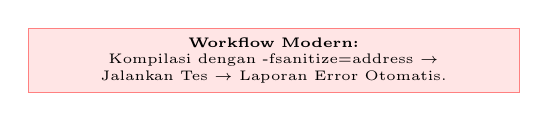
\begin{tikzpicture}[
        node/.style={rectangle, draw=red!50, fill=red!10, text width=6cm, font=\tiny, align=center}
    ]
    \node[node] (asan) {
        \textbf{Workflow Modern:}\\
        Kompilasi dengan \code{-fsanitize=address} $\rightarrow$ Jalankan Tes $\rightarrow$ Laporan Error Otomatis.
    };
    \end{tikzpicture}%
    }
    \caption{Debugging Cepat menggunakan Sanitizers}
\end{figure}

\section{Performance Analysis}

\subsection{FlameGraphs: Visualisasi Bottleneck}
Kompilator adalah aplikasi yang sangat haus sumber daya. Untuk mengidentifikasi fungsi mana yang paling lambat, pengembang menggunakan \compiler{FlameGraphs}.
\begin{itemize}
    \item \textbf{Visual}: Memberikan representasi visual dari pohon panggilan (\textit{call stacks}). Semakin lebar sebuah kotak, semakin banyak waktu CPU yang dihabiskan dalam fungsi tersebut.
    \item \textbf{Manfaat}: Memungkinkan identifikasi instan terhadap bagian optimasi kompilator yang terlalu membebani performa.
\end{itemize}

\subsection{Infrastruktur: Reproducible Builds}
Dalam proyek kompilator skala besar, konsistensi lingkungan sangat penting.
\begin{itemize}
    \item \textbf{Docker}: Digunakan untuk membungkus seluruh \textit{toolchain} kompilator agar setiap pengembang dan server CI/CD menggunakan versi GCC/LLVM, Flex, dan Bison yang identik. Hal ini menjamin biner yang dihasilkan selalu konsisten (\textit{reproducible}).
\end{itemize}

\begin{figure}[!htbp]
    \centering
    \adjustbox{max width=0.8\textwidth,center}{%
    \begin{tikzpicture}[
        rect/.style={rectangle, draw=orange!50, fill=orange!10, text width=5cm, align=center, font=\tiny}
    ]
    \node[rect] (p) {Profiling (Perf/Gprof)};
    \node[rect, below=0.2cm of p] (f) {Visualization (FlameGraphs)};
    \node[rect, below=0.2cm of f] (o) {Optimization (Refactor hot spots)};
    \draw[->] (p) -- (f);
    \draw[->] (f) -- (o);
    \end{tikzpicture}%
    }
    \caption{Siklus Optimasi Performa Kompilator}
\end{figure}


% ============================================================
% AKTIVITAS PEMBELAJARAN
% ============================================================
\begin{aktivitas}
  \item \textbf{Flex/Bison}: Buat simple calculator menggunakan Flex dan Bison.
  \item \textbf{ANTLR}: Implementasikan parser untuk bahasa ekspresi dengan ANTLR.
  \item \textbf{LLVM}: Buat LLVM pass untuk optimasi sederhana.
  \item \textbf{Build Systems}: Konversi Makefile ke CMake.
  \item \textbf{Debugging}: Debug compiler crash dengan GDB.
\end{aktivitas}

% ============================================================
% LATIHAN DAN REFLEKSI
% ============================================================
\begin{latihan}
  \item Bandingkan Flex dan re2c untuk lexer generation!
  \item Implementasikan parser untuk bahasa dengan control structures menggunakan Bison!
  \item Analisis LLVM IR untuk program sederhana!
  \item Konversi build system dari Make ke CMake untuk project compiler!
  \item Debug memory leak dalam parser generator!
  \item \textbf{Refleksi}: Bagaimana compiler tools mempengaruhi produktivitas pengembangan compiler?
\end{latihan}

% ============================================================
% ASESMEN
% ============================================================
\begin{asesmen}
\textbf{Instrumen Penilaian untuk Sub-CPMK 6.1}

\textbf{A. Pilihan Ganda}

\begin{enumerate}
  \item Flex adalah:
  \begin{enumerate}
    \item Parser generator
    \item Lexer generator
    \item Build system
    \item Debugger
  \end{enumerate}
  
  \item Bison menggunakan parsing algorithm:
  \begin{enumerate}
    \item LL(1)
    \item LR(1)
    \item LALR(1)
    \item Recursive descent
  \end{enumerate}
  
  \item LLVM adalah:
  \begin{enumerate}
    \item Compiler framework
    \item Build system
    \item Debugger
    \item Lexer generator
  \end{enumerate}
\end{enumerate}

\textbf{B. Essay}

\begin{enumerate}
  \item Jelaskan ekosistem compiler tools dan peran masing-masing tool!
  \item Implementasikan mini compiler menggunakan Flex, Bison, dan build system modern!
\end{enumerate}

\textbf{Rubrik Penilaian}: Lihat Lampiran A
\end{asesmen}

% ============================================================
% CHECKLIST KOMPETENSI
% ============================================================
\begin{checklist}
  \item Saya dapat menganalisis dan menggunakan compiler tools modern
  \item Saya dapat menggunakan lexer generators (Flex, re2c)
  \item Saya dapat menggunakan parser generators (Bison, ANTLR)
  \item Saya memahami compiler frameworks (LLVM, GCC)
  \item Saya dapat menggunakan build systems (Make, CMake)
  \item Saya dapat menggunakan debugging tools untuk compiler development
\end{checklist}

% ============================================================
% RANGKUMAN
% ============================================================
\begin{rangkuman}
Bab ini membahas compiler tools analysis, termasuk lexer generators, parser generators, compiler frameworks, build systems, dan debugging tools. Mahasiswa belajar menggunakan tools modern untuk pengembangan compiler yang efisien.

\textbf{Poin Kunci:}
\begin{itemize}
  \item Compiler tools menyederhanakan pengembangan compiler
  \item Lexer generators otomatisasi token recognition
  \item Parser generators menghasilkan efficient parsers
  \item Compiler frameworks menyediakan infrastructure lengkap
  \item Build systems mengelola compilation dependencies
  \item Debugging tools membantu identifikasi dan perbaikan bugs
\end{itemize}

\textbf{Kata Kunci}: \compiler{Compiler Tools}, \compiler{Flex}, \compiler{Bison}, \compiler{ANTLR}, \compiler{LLVM}, \compiler{GCC}, \compiler{Make}, \compiler{CMake}, \compiler{GDB}, \compiler{Valgrind}
\end{rangkuman}

\ifSubfilesClassLoaded{%
    \clearpage
    \printbibliography[title={Daftar Pustaka}]
    \end{refsection}
}{}

\end{document}
